\documentclass[11pt,a4paper]{article} 
\usepackage{listings}
\usepackage{xcolor}

\definecolor{codegreen}{rgb}{0,0.6,0}
\definecolor{codegray}{rgb}{0.5,0.5,0.5}
\definecolor{codepurple}{rgb}{0.58,0,0.82}
% \definecolor{codepurple}{RGB}{245, 51, 55}
\definecolor{backcolour}{RGB}{231, 230, 237}

\lstdefinestyle{mystyle}{
    backgroundcolor=\color{backcolour},   
    commentstyle=\color{codegreen},
    keywordstyle=\color{red},
    numberstyle=\tiny\color{codegray},
    stringstyle=\color{blue},
    basicstyle=\ttfamily\footnotesize,
    breakatwhitespace=false,         
    breaklines=true,                 
    captionpos=b,                    
    keepspaces=true,                 
    % numbers=left,                    
    numbersep=5pt,                  
    showspaces=false,                
    showstringspaces=false,
    showtabs=false,                  
    tabsize=2
}

\lstset{style=mystyle}
\usepackage{titlesec}
\usepackage{color}
\usepackage[utf8]{inputenc}
\usepackage[english]{babel}
\usepackage[T1]{fontenc}
\usepackage{graphicx}
\graphicspath{{Images/}}
\usepackage{eso-pic} 
\usepackage{subfig} 
\usepackage{caption}
\usepackage{transparent}
\usepackage{graphicx}
\graphicspath{ {./Images/} }

% STANDARD MATH PACKAGES
\usepackage{amsmath}
\usepackage{amsthm}
\usepackage{bm}
\usepackage[overload]{empheq} 

% PACKAGES FOR TABLES
\usepackage{tabularx}
\usepackage{colortbl}
\usepackage{mathtools}  

% PACKAGES FOR ALGORITHMS (PSEUDO-CODE)
\usepackage{algorithm}
\usepackage{algorithmic}

% PACKAGES FOR REFERENCES & BIBLIOGRAPHY
\usepackage[colorlinks=true,linkcolor=black,anchorcolor=black,citecolor=black,filecolor=black,menucolor=black,runcolor=black,urlcolor=black]{hyperref} % Adds clickable links at references
\usepackage{cleveref}
\usepackage[square, numbers, sort&compress]{natbib} 

\bibliographystyle{plain} % You may use a different style adapted to your field

% PACKAGES FOR THE APPENDIX
\usepackage{appendix}

% PACKAGES FOR ITEMIZE & ENUMERATES 
\usepackage{enumitem}

% OTHER PACKAGES
\usepackage{amsthm,thmtools,xcolor} % Coloured "Theorem"
\usepackage{fancyhdr} % Fancy headers and footers
\usepackage{lipsum} % Insert dummy text
\usepackage{tcolorbox} % Create coloured boxes



% Do not change Configuration_files/config.tex file unless you really know what you are doing.
%DO NOT EDIT
% Configuration package
\usepackage[bottom=2.0cm,top=2.0cm,left=2.0cm,right=2.0cm]{geometry}
\raggedbottom 

\definecolor{newblue}{cmyk}{0.4,0.1,0,0.4}

% Custom theorem environments
\declaretheoremstyle[
  headfont=\color{newblue}\normalfont\bfseries,
  bodyfont=\color{black}\normalfont\itshape,
]{colored}

\captionsetup[figure]{labelfont={color=newblue}} 
\captionsetup[table]{labelfont={color=newblue}} 
\captionsetup[algorithm]{labelfont={color=newblue}} 

\theoremstyle{colored}
\newtheorem{theorem}{Theorem}[section]
\newtheorem{proposition}{Proposition}[section]

\newcommand\T{\rule{0pt}{2.6ex}}
\newcommand\B{\rule[-1.2ex]{0pt}{0pt}}

\newcounter{algsubstate}
\renewcommand{\thealgsubstate}{\alph{algsubstate}}
\newenvironment{algsubstates}{
    \setcounter{algsubstate}{0}%
    \renewcommand{\STATE}{%
    \stepcounter{algsubstate}%
    \Statex {\small\thealgsubstate:}\space}
    }{}
    
% Custom theorem environment
\newcolumntype{L}[1]{>{\raggedright\let\newline\\\arraybackslash\hspace{0pt}}m{#1}}
\newcolumntype{C}[1]{>{\centering\let\newline\\\arraybackslash\hspace{0pt}}m{#1}}
\newcolumntype{R}[1]{>{\raggedleft\let\newline\\\arraybackslash\hspace{0pt}}m{#1}}

% Custom itemize environment
\setlist[itemize,1]{label=$\bullet$}
\setlist[itemize,2]{label=$\circ$}
\setlist[itemize,3]{label=$-$}
\setlist{nosep}


\setlength\parindent{0pt}

% Custom title commands
\titleformat{\section}
{\color{newblue}\normalfont\Large\bfseries}
{\color{newblue}\thesection.}{1em}{}
\titlespacing*{\section}
{0pt}{3.3ex}{3.3ex}

\titleformat{\subsection}
{\color{newblue}\normalfont\large\bfseries}
{\color{newblue}\thesubsection.}{1em}{}
\titlespacing*{\subsection}
{0pt}{3.3ex}{3.3ex}

% Custom headers and footers
\pagestyle{fancy}
\fancyhf{}
      
\fancyfoot{}
\fancyfoot[C]{\thepage} % page
\renewcommand{\headrulewidth}{0mm} % headrule width
\renewcommand{\footrulewidth}{0mm} % footrule width

\makeatletter
\patchcmd{\headrule}{\hrule}{\color{black}\hrule}{}{} % headrule
\patchcmd{\footrule}{\hrule}{\color{black}\hrule}{}{} % footrule
\makeatother

% Insert here the info that will be displayed into your Title page 
\renewcommand{\title}{\textcolor{blue}{Graph Template Library}}
\newcommand{\authorA}{Atharva Suhas Mulay (2021CSB1076)}
\newcommand{\authorB}{Karanraj Mehta (2021CSB1100)}
\newcommand{\authorC}{Sumit Patil (2021CSB1135)} %comment if not needed
%\newcommand{\authorD}{Student4Name (ID4)} %comment if not needed
\newcommand{\advisor}{Dr. Anil Shukla}
\newcommand{\firstcoadvisor}{Sravanti Chede}
\newcommand{\summary}{  
\begin{itemize}  
\item[--] Graph template library to study graphs in C++
\item[--] Generic graph library
\item[--] Defines several container template classes
\item[--] Data structures for graphs, digraphs and weighted graphs
\item[--] Many standard graph algorithms
\item[--] Nodes can be arbitrary objects
\end{itemize}  
}

%-------------------------------------------------------------------------
%	BEGIN OF YOUR DOCUMENT
%-------------------------------------------------------------------------
\begin{document}

% Do not change Configuration_files/TitlePage.tex
% DO NOT EDIT


\null\hfill
\includegraphics[width=0.2\textwidth]{Images/IIT_Rpr_logo.jpg}

\vspace{3mm}
\Large{\textbf{\color{newblue}{\title}}}
\vspace{0.1cm}\\
\null\hfill \today\\
\large{\textbf{\authorA}}\vspace{1mm}
,\\ \large{\textbf{\authorB}}\vspace{1mm}
\ifdefined \authorC
,\\ \large{\textbf{\authorC}}\vspace{1mm}
\ifdefined \authorD
,\\ \large{\textbf{\authorD}}\vspace{1mm}
\fi 
\fi
\small \normalfont

\vspace{11pt}

\centerline{\rule{1.0\textwidth}{0.4pt}}

\begin{center}
\begin{minipage}[t]{.24\textwidth}
\begin{minipage}{.90\textwidth}
\noindent
\footnotesize{\textbf{Instructor:} \\
\advisor} \\
\\
\footnotesize{\textbf{Teaching Assistant:}\\ 
\firstcoadvisor}\\ 

\end{minipage}
\end{minipage}
\begin{minipage}{.74\textwidth}
\noindent \textbf{\color{newblue} Summary:} {\summary}
\end{minipage}
\end{center}

\vspace{8pt}

\centerline{\rule{1.0\textwidth}{0.4pt}}
\vspace{12pt}
%Main Text starting point
\section*{\textcolor{red}{Introduction}}
\label{sec:introduction}
An Abstract Data Type in data structures is a kind of data type whose behaviour is defined with the help of some attributes and some functions. Generally, we write these attributes and functions inside a class or a structure so that we can use an object of the class to use that particular abstract data type. Graph is an abstract data structure. They are mathematical data structures that are useful for solving many kinds of problems in computer science
\\
\\
A graph is a relation on a finite set of vertices. Two vertices are related if there is an edge between them. If V and E denote the set of vertices and edges, the graph is represented as G(V, E).

\\
\\
There are several types of graphs in data structures. These include undirected, directed, weighted, multi, complete, simple, bipartite, and cyclic graphs. In our library, we have focused mainly on weighted and unweighted directed and undirected graphs.
\\
\begin{itemize}  
\item[--] Unweighted Graph: No value associated with the edges
\item[--] Weighted Graph: Whose edges have values. All the values associated with the edges are called weights.
\item[--] Undirected Graph: All edges are bidirectional
\item[--] Directed Graph: All edges are directed from one node to the other.
\\
\end{itemize}  

Graphs can be represented using either an Adjacency list or an Adjacency matrix. In our library, we’ve used adjacency list representation of graphs because it is more space efficient. In the adjacency list representation, each node is mapped to a list of all its adjacencies or neighbours.
\\
\\
All classes, functions and variable names are lower\_case\_underscore. Our library provides the following graph types:
\\
\begin{itemize}  
\item[--] \begin{verbatim}
graph
\end{verbatim}

This class implements an undirected graph. It assumes multiple edges between two nodes are not added. It does allow self-loop edges between a node and itself.

\item[--]\begin{verbatim}
digraph
\end{verbatim} 

Directed graphs, that is, graphs with directed edges. Provides operations common to directed graphs.

\item[--] \begin{verbatim}
wgraph
\end{verbatim}

Weighted undirected graphs. Allows only integer weights to the edges.
\item[--] \begin{verbatim}
wdigraph
\end{verbatim}

Weighted directed graphs. Allows only integer weights to the edges.
\\
\end{itemize}  
All graph classes allow any object as node such as \texttt{char, int, string }and more. Only int weights are allowed in wgraph and wdigraph classes.
\\
\\
The graph internal data structures are based on an adjacency list representation and implemented using map data structures. In unweighted graphs, each node in the adjacency list is mapped to a list (vector) of its neighbours. In weighted graphs, each node is mapped to a vector of pairs in which the first attribute is the neighbour of that node and the second attribute is the weight of the edge connecting it to that node.

\\
\\
% \begin{verbatim}
% \section{Title of the section}
% \end{verbatim}
% The numbering can be turned off by using \verb|\section*{}|.
% A new subsection is created by the command
% \begin{verbatim}
% \subsection{Title of the subsection}
% \end{verbatim}
% and, similarly, the numbering can be turned off by adding an asterisk as follows 
% \begin{verbatim}
% \subsection*{}
% \end{verbatim}
% It is recommended to give a label to each section by using the command
% \begin{verbatim}
% \label{sec:section_name}%
% \end{verbatim}
% where the argument is just a text string that you'll use to reference that part
% as follows: \textit{Section~\ref{sec:introduction} contains \sc{INTRODUCTION}  \dots}.
% \documentclass{beamer}


\subsection*{\textcolor{blue}{\Large Example }}

% \rule{17cm}{0.1mm}


Finds number of connected components in an undirected graph
\begin{lstlisting}[language=C++]
 #include <iostream>
 #include "graph.h"

  int main() {
    graph<char> g;
    g.add_edge('a', 'b');
    g.add_edge('c', 'd');
    g.add_edge('d', 'e');
    g.add_edge('f', 'g');

    std::cout << "Number of connected components in g are " << g.number_of_connected_components() << "\n";
    return 0;
   }   

\end{lstlisting}
\\
{\textcolor{black}{\normalsize Output }}
\begin{lstlisting}[language=C++]
Number of connected components in g are 3
\end{lstlisting}
\rule{17cm}{0.5mm}
\section*{\textcolor{blue}{{\huge \texttt{graph} Class}} }
A template container class for unweighted undirected graphs. Self-loops are allowed, but multiple edges are not. Nodes can be arbitrary objects.

\subsection*{\textcolor{blue}{{\LARGE - Members}}}
% \rule{17cm}{0.1mm}
\subsubsection*{\textcolor{blue}{ \Large \texttt{graph::number\_of\_edges}}}
Stores number edges in the graph
\subsubsection*{\textcolor{blue}{ \large{Syntax}}}
\begin{lstlisting}[language=C++]
 int number_of_edges;
\end{lstlisting}
\subsubsection*{\textcolor{blue}{ \large{Remarks}}}
The member variable is 0 for an empty graph

\rule{17cm}{0.1mm}



\subsubsection*{\textcolor{blue}{ \Large \texttt{graph::adj}}}
Stores the adjacency list of the graph. It is implemented using map data structure in which each node is mapped to a vector to its neighbours.

\subsubsection*{\textcolor{blue}{ \large {Syntax}}}
\begin{lstlisting}[language=C++]
 std::map<T, std::vector<T>> adj;
\end{lstlisting}
T is a template parameter
\\
\rule{17cm}{0.1mm}




\subsubsection*{\textcolor{blue}{ \Large \texttt{graph::add\_node}}}
Adds the specified node to that graph
\subsubsection*{\textcolor{blue}{ \large {Syntax}}}
\begin{lstlisting}[language=C++]
 void add_node(T u);
\end{lstlisting}
\subsubsection*{\textcolor{blue}{ \large {Parameters}}}
u\\
Node to be added
\subsubsection*{\textcolor{blue}{ \large {Time Complexity}}}
O(log n) worst case time complexity where n is the number of nodes since the adjacency list uses map data structure which takes O(log n) time for insertion.
\\
\rule{17cm}{0.1mm}



\subsubsection*{\textcolor{blue}{ \Large \texttt{graph::add\_edge
}}}
Adds an undirected edge between the two specified nodes.

\subsubsection*{\textcolor{blue}{ \large {Syntax}}}
\begin{lstlisting}[language=C++]
 void add_edge(T u, T v)

\end{lstlisting}
\subsubsection*{\textcolor{blue}{ \large {Parameters}}}
u\\
First node\\
v\\
Second node
\subsubsection*{\textcolor{blue}{ \large {Remarks}}}
It is assumed that multiple edges between two nodes are not added.


\subsubsection*{\textcolor{blue}{ \large {Time Complexity}}}
O(log n) where n is the number of nodes.
\\
\rule{17cm}{0.1mm}



\subsubsection*{\textcolor{blue}{ \Large \texttt{graph::number\_of\_nodes}}}

Returns the number of nodes in the graph

\subsubsection*{\textcolor{blue}{ \large {Syntax}}}
\begin{lstlisting}[language=C++]
 int number_of_nodes();

\end{lstlisting}
\subsubsection*{\textcolor{blue}{ \large {Return Value
}}}
Number of nodes in the graph

\subsubsection*{\textcolor{blue}{ \large {Time Complexity}}}
O(1)
\\
\rule{17cm}{0.1mm}


\subsubsection*{\textcolor{blue}{ \Large \texttt{graph::remove\_node}}}
Removes the specified node from the graph

\subsubsection*{\textcolor{blue}{ \large {Syntax}}}
\begin{lstlisting}[language=C++]
 void remove_node(T u);

\end{lstlisting}
\subsubsection*{\textcolor{blue}{ \large {Parameters
}}}
u
Node to be removed


\subsubsection*{\textcolor{blue}{ \large {Time Complexity}}}
O($n^2$ log n) worst case time complexity assuming complete graph where n is the number of vertices
\\
\rule{17cm}{0.1mm}



\subsubsection*{\textcolor{blue}{ \Large \texttt{graph::remove\_edge}}}
Removes the specified edge from the graph

\subsubsection*{\textcolor{blue}{ \large {Syntax}}}
\begin{lstlisting}[language=C++]
 void remove_edge(T u, T v);

\end{lstlisting}
\subsubsection*{\textcolor{blue}{ \large {Parameters
}}}
u, v nodes between which the edge is to be removed


\subsubsection*{\textcolor{blue}{ \large {Time Complexity}}}
O($n$) 
\\
\rule{17cm}{0.1mm}


\subsubsection*{\textcolor{blue}{ \Large \texttt{graph::degree}}}
Returns the degree of the specified node

\subsubsection*{\textcolor{blue}{ \large {Syntax}}}
\begin{lstlisting}[language=C++]
int degree(T u);

\end{lstlisting}
\subsubsection*{\textcolor{blue}{ \large {Parameters
}}}
u \\
Node whose degree is to be found



\subsubsection*{\textcolor{blue}{ \large {Time Complexity}}}
O(log n)
\\
\rule{17cm}{0.1mm}


\subsubsection*{\textcolor{blue}{ \Large \texttt{graph::clear}}}
Empties the graph

\subsubsection*{\textcolor{blue}{ \large {Syntax}}}
\begin{lstlisting}[language=C++]
void clear();

\end{lstlisting}
\subsubsection*{\textcolor{blue}{ \large {Time Complexity}}}
O(log n)
\\
\rule{17cm}{0.1mm}
\subsubsection*{\textcolor{blue}{\Large\texttt{graph::number\_of\_connected\_components}}}
Finds the number of connected components in the graph


\subsubsection*{\textcolor{blue}{ \large {Syntax}}}
\begin{lstlisting}[language=C++]
int number_of_connected_components();
\end{lstlisting}
\subsubsection*{\textcolor{blue}{ \large {Return Value}}}
Returns the number of connected components in the graph



\subsubsection*{\textcolor{blue}{ \large {Algorithm}}}
This function calculates the number of connected components by running a series of DFS.
\begin{enumerate}  
\item Start at one node and perform DFS. All nodes in the connected component containing this node will be found.
\item Find the next unvisited node and run DFS on it, finding the second connected component.
\item If some unvisited nodes are still left, continue from step 2.
\item Finally, return the number of connected components.

 \end{enumerate}  

\subsubsection*{\textcolor{blue}{ \large {Time Complexity}}}
Since this algorithm will not run on the same vertex twice, its time complexity will be same as that of dfs, that is O(V log V + E)



\\
\rule{17cm}{0.1mm}

\subsection*{\textcolor{blue}{\Large Example }}

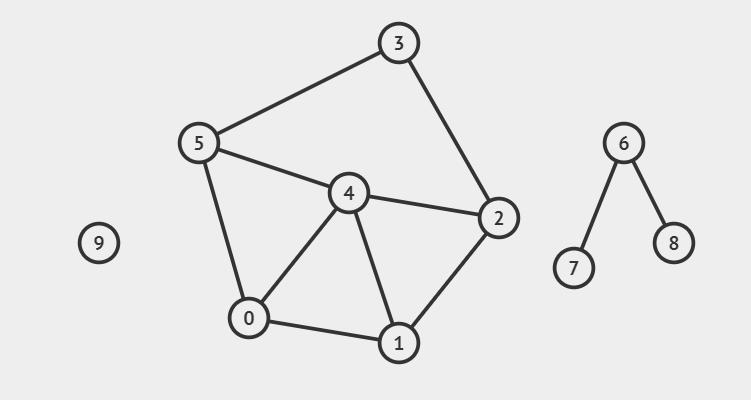
\includegraphics[width=70mm]{example1}
\begin{lstlisting}[language=C++]
 #include <iostream>
#include "graph.h"

int main() {
    graph<int> g;
    g.add_edge(0, 1);
    g.add_edge(0, 4);
    g.add_edge(0, 5);
    g.add_edge(1, 2);
    g.add_edge(1, 4);
    g.add_edge(2, 3);
    g.add_edge(2, 4);
    g.add_edge(3, 5);
    g.add_edge(4, 5);
    g.add_edge(6, 7);
    g.add_edge(6, 8);

    g.add_node(9);

    
    std::cout<<"The Number of Nodes is : "<<g.number_of_nodes()<<std::endl;
    std::cout<<"The Number of Edges is : "<<g.number_of_edges<<std::endl;
    std::cout<<"The Number of Connected Components is : "<<g.number_of_connected_components()<<std::endl;
    std::cout<<"The Degree of 4 is : "<<g.degree(4)<<std::endl;
    std::map<int,std::vector<int>>M= g.adj;
    std::cout<<"\n";
    std::cout<<"The Adjacency List is : "<<std::endl;
    
    for(auto it:g.adj){
        std::cout<<it.first<<" : ";
        for(auto i:it.second){
            std::cout<<i<<" ";
        }
        std::cout<<std::endl;
    }


    
    return 0;
}

\end{lstlisting}
\\
{\textcolor{black}{\normalsize Output }}
\begin{lstlisting}[language=C++]
The Number of Nodes is : 10
The Number of Edges is : 11
The Number of Connected Components is : 3
The Degree of 4 is : 4

The Adjacency List is :
0 : 1 4 5
1 : 0 2 4
2 : 1 3 4
3 : 2 5
4 : 0 1 2 5
5 : 0 3 4
6 : 7 8
7 : 6
8 : 6
9 :

\end{lstlisting}
\rule{17cm}{0.1mm}

\subsubsection*{\textcolor{blue}{ \Large \texttt{graph::bfs}}}
It performs Breadth-First Search traversal on a given graph with given source vertex s.



\subsubsection*{\textcolor{blue}{ \large {Syntax}}}
\begin{lstlisting}[language=C++]
std::vector<T> bfs(T s);


\end{lstlisting}
\subsubsection*{\textcolor{blue}{ \large {Parameters
}}}
s\\
Source vertex

\subsubsection*{\textcolor{blue}{ \large {Return Value}}}
Returns a vector containing the bfs traversal starting from source vertex s.

\subsubsection*{\textcolor{blue}{ \large {Algorithm}}}
The BFS algorithm is defined as follows:
\begin{enumerate}  
\item Consider an undirected graph with vertices numbered from 1 to n. Initialise queue q as a new queue containing only vertex s, and mark the vertex s as visited.

 
\item Extract a vertex v from the head of the queue q.

\item Store vertex v in bfs traversal.

\item Iterate in arbitrary order through all such vertices u that u is a neighbour of v and is not marked yet as visited. Mark the vertex u as visited and insert it into the tail of the queue q.
\item If the queue is not empty, continue from step 2.
\item Otherwise, return the bfs traversal of the graph.
\end{enumerate}  

\subsubsection*{\textcolor{blue}{ \large {Time Complexity}}}
For regular bfs, the time complexity is O(V + E), where V is the number of vertices and E is the number of edges. However, because of the map implementation of the adjacency list, it becomes O(V log V + E)


\\
\rule{17cm}{0.1mm}



\subsubsection*{\textcolor{blue}{ \Large \texttt{graph::dfs}}}
It performs Depth First Search traversal on a given graph with a given source vertex u.

\subsubsection*{\textcolor{blue}{ \large {Syntax}}}
\begin{lstlisting}[language=C++]
std::vector<T> dfs(T u);


\end{lstlisting}
\subsubsection*{\textcolor{blue}{ \large {Parameters
}}}
u\\
Source vertex


\subsubsection*{\textcolor{blue}{ \large {Return Value}}}
Returns a vector containing the dfs traversal starting from source vertex u.


\subsubsection*{\textcolor{blue}{ \large {Algorithm}}}
The recursive implementation of DFS is as follows:

\begin{enumerate}  
\item Start the search at one vertex.
\item After visiting that vertex, we perform a DFS for each adjacent vertex we haven't visited before.
\item This way, we visit all vertices that are reachable from the starting vertex.

\end{enumerate}  
The iterative implementation of DFS is as follows:
\begin{enumerate}  
\item Initialise stack s as a new stack containing only vertex u, and mark the vertex u as visited.
\item Extract v from the top of the stack s.

\item Store vertex v in the dfs traversal.
\item Iterate in arbitrary order through all such vertices u that u is a neighbour of v and is not marked yet as visited. Mark the vertex u as visited and push it into the stack s.
\item If the stack is not empty, continue from step 2.
\item Otherwise, return the dfs traversal of the graph.

\end{enumerate} 
\subsubsection*{\textcolor{blue}{ \large {Time Complexity}}}
O(V log V + E)
\\
\rule{17cm}{0.1mm}





\subsubsection*{\textcolor{blue}{\Large\texttt{graph::cyclic}}}
Checks whether the graph contains a cycle or not
\subsubsection*{\textcolor{blue}{ \large {Syntax}}}
\begin{lstlisting}[language=C++]
bool cyclic();
\end{lstlisting}
\subsubsection*{\textcolor{blue}{ \large {Return Value}}}
Returns true if the graph is cyclic, else returns false
\subsubsection*{\textcolor{blue}{ \large {Algorithm}}}
It uses DFS to check for cyclicity.

\begin{enumerate}  
\item Initially all vertices are unvisited.
\item Construct a data structure to store parents (In our implementation, we use a map).
\item For each unvisited node, run DFS and update the parent map.
\item If DFS discovers a visited node, then we have found a cycle and return true.

\item Otherwise return false.
\end{enumerate}  
The parent map can be used the print the cycle found.


\subsubsection*{\textcolor{blue}{ \large {Time Complexity}}}
Since this algorithm will not run on the same vertex twice, its time complexity will be same as that of dfs, that is O(V log V + E)

\\
\rule{17cm}{0.1mm}


\subsection*{\textcolor{blue}{\Large Example }}
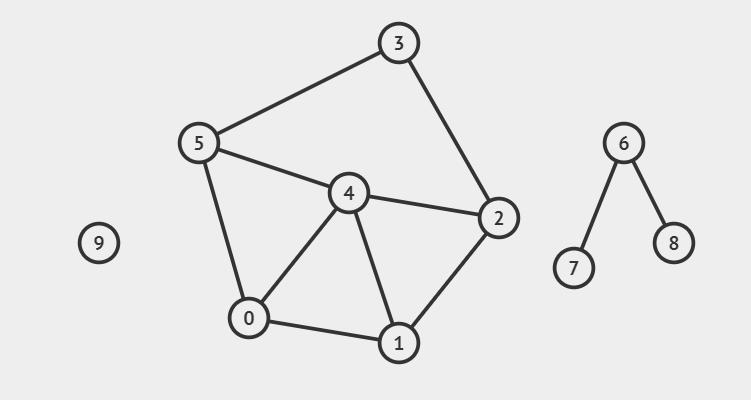
\includegraphics[width=70mm]{example2.png}
\begin{lstlisting}[language=C++]
 #include <iostream>
#include "graph.h"

int main()
{
    graph<int> g;
    g.add_edge(0, 1);
    g.add_edge(0, 4);
    g.add_edge(0, 5);
    g.add_edge(1, 2);
    g.add_edge(1, 4);
    g.add_edge(2, 3);
    g.add_edge(2, 4);
    g.add_edge(3, 5);
    g.add_edge(4, 5);
    g.add_edge(6, 7);
    g.add_edge(6, 8);

    g.add_node(9);

    std::vector<int> V1 = g.dfs(0);
    std::vector<int> V2 = g.bfs(0);
    std::cout << "The DFS Traversal is : ";
    for (auto it : V1)
    {
        std::cout << it << " ";
    }
    std::cout << std::endl;
    std::cout << "The BFS Traversal is : ";
    for (auto it : V2)
    {
        std::cout << it << " ";
    }
    std::cout << std::endl;

    if (g.cyclic())
    {
        std::cout<<"Graph has atleast one cycle."<<std::endl;
    }
    else{
        std::cout<<"Graph doesn't have a cycle"<<std::endl;
    }
    return 0;
}

\end{lstlisting}
\\
{\textcolor{black}{\normalsize Output }}
\begin{lstlisting}[language=C++]
The DFS Traversal is : 0 5 3 2 4 1 
The BFS Traversal is : 0 1 4 5 2 3 
Graph has atleast one cycle.

\end{lstlisting}
\rule{17cm}{0.1mm}
\subsubsection*{\textcolor{blue}{\Large\texttt{graph::is\_bipartite}}}
Checks whether the graph is bipartite or not
\subsubsection*{\textcolor{blue}{ \large {Syntax}}}
\begin{lstlisting}[language=C++]
bool is_bipartite();
\end{lstlisting}
\subsubsection*{\textcolor{blue}{ \large {Return Value}}}
Returns true if the graph is bipartite, else returns false
\subsubsection*{\textcolor{blue}{ \large {Algorithm}}}
The algorithm uses the fact that a graph is bipartite if and only if it is two-colorable. Here, use BFS to traverse the graph.
\begin{enumerate}  
\item For each unvisited vertex assign it one colour, say blue and assign all it’s neighbours the opposite colour, say red.
\item When the neighbour of a vertex has already been visited, we check whether its colour is opposite to the current node or not. If yes, continue from step 1, else return false.
\item Finally if all the vertices have been visited, we conclude that the graph is bipartite and return true.
 

\end{enumerate}  

\subsubsection*{\textcolor{blue}{ \large {Time Complexity}}}
Since this algorithm will not run on the same vertex twice, its time complexity will be same as that of bfs, that is O(V log V + E)

\\
\rule{17cm}{0.1mm}
\subsection*{\textcolor{blue}{\Large Example }}
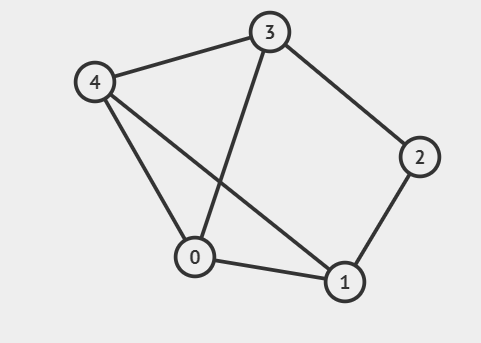
\includegraphics[width=70mm]{example3 (3).png}
\\
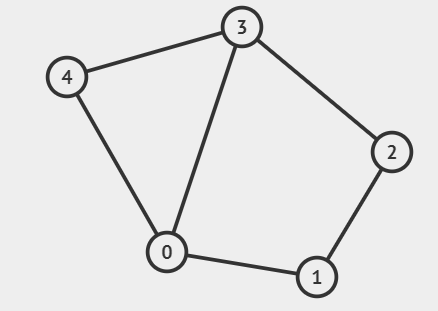
\includegraphics[width=70mm]{example3 (2).png}
\\
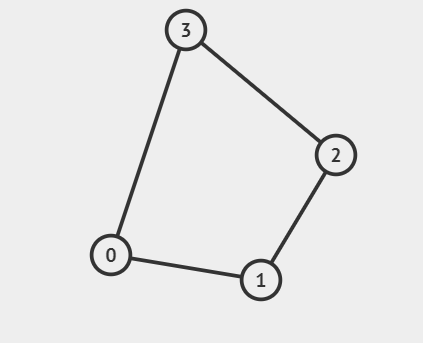
\includegraphics[width=70mm]{example3 (1).png}
\begin{lstlisting}[language=C++]
#include <iostream>
#include "graph.h"

int main()
{
    graph<int> g;
    g.add_edge(0, 1);
    g.add_edge(0, 3);
    g.add_edge(0, 4);
    g.add_edge(1, 2);
    g.add_edge(2, 3);
    g.add_edge(3, 4);
    g.add_edge(4, 1);

    std::cout << "The Adjacency List is : " << std::endl;

    for (auto it : g.adj)
    {
        std::cout << it.first << " : ";
        for (auto i : it.second)
        {
            std::cout << i << " ";
        }
        std::cout << std::endl;
    }
    std::cout << std::endl;
    if (g.is_bipartite())
    {
        std::cout << "The Graph is Bipartite" << std::endl;
    }
    else
    {
        std::cout << "The Graph is not Bipartite" << std::endl;
    }
    g.remove_edge(4, 1);
    std::cout << std::endl;
    std::cout << "The Adjacency List after removing edge between 4 and 1 is : " << std::endl;

    for (auto it : g.adj)
    {
        std::cout << it.first << " : ";
        for (auto i : it.second)
        {
            std::cout << i << " ";
        }
        std::cout << std::endl;
    }

    g.remove_node(4);
    std::cout << std::endl;
    std::cout << "The Adjacency List after removing node 4 is : " << std::endl;

    for (auto it : g.adj)
    {
        std::cout << it.first << " : ";
        for (auto i : it.second)
        {
            std::cout << i << " ";
        }
        std::cout << std::endl;
    }

    if (g.is_bipartite())
    {
        std::cout << "The Graph is Bipartite" << std::endl;
    }
    else
    {
        std::cout << "The Graph is not Bipartite" << std::endl;
    }
    return 0;
}

\end{lstlisting}
\\
{\textcolor{black}{\normalsize Output }}
\begin{lstlisting}[language=C++]
The Adjacency List is : 
0 : 1 3 4 
1 : 0 2 4 
2 : 1 3 
3 : 0 2 4 
4 : 0 3 1 

The Graph is not Bipartite

The Adjacency List after removing edge between 4 and 1 is : 
0 : 1 3 4 
1 : 0 2
2 : 1 3
3 : 0 2 4
4 : 0 3

The Adjacency List after removing node 4 is :
0 : 1 3
1 : 0 2
2 : 1 3
3 : 0 2

The Graph is Bipartite.
\end{lstlisting}
\rule{17cm}{0.1mm}
\section*{\textcolor{blue}{{\huge \texttt{digraph} Class}} }
A template container class for unweighted directed graphs. Self-loops are allowed, but multiple edges (parallel) are not. Nodes can be arbitrary objects.

\subsection*{\textcolor{blue}{{\LARGE - Members}}}
For number\_of\_edges, adj, add\_node, number\_f\_nodes, remove\_node, clear, bfs, dfs see graph class.

\rule{17cm}{0.1mm}


\subsubsection*{\textcolor{blue}{\Large\texttt{digraph::add\_edge}}}
Adds a directed edge from the first node to the second
\subsubsection*{\textcolor{blue}{ \large {Syntax}}}
\begin{lstlisting}[language=C++]
void add_edge(T u, T v);
\end{lstlisting}
\subsubsection*{\textcolor{blue}{ \large {Parameters}}}
u \\
First node
v\\
Second node

\subsubsection*{\textcolor{blue}{ \large {Remarks}}}
Edge is directed from u to v (first node to second). It is assumed that multiple edges between two nodes are not added. The order in which the nodes occur is important.



\subsubsection*{\textcolor{blue}{ \large {Time Complexity}}}
O(log n)
\\
\rule{17cm}{0.1mm}

\subsubsection*{\textcolor{blue}{\Large\texttt{digraph::remove\_edge}}}
Removes the specified edge from the graph
\subsubsection*{\textcolor{blue}{ \large {Syntax}}}
\begin{lstlisting}[language=C++]
void remove_edge(T u, T v);

\end{lstlisting}
\subsubsection*{\textcolor{blue}{ \large {Parameters}}}
u, v nodes between which the edge is to be removed


\subsubsection*{\textcolor{blue}{ \large {Remarks}}}
The order in which the nodes occur is important.


\subsubsection*{\textcolor{blue}{ \large {Time Complexity}}}
O(n)

\\
\rule{17cm}{0.1mm}

\subsubsection*{\textcolor{blue}{\Large\texttt{digraph::in\_degree}}}
Stores the in degree of all nodes in the graph
\subsubsection*{\textcolor{blue}{ \large {Syntax}}}
\begin{lstlisting}[language=C++]
std::map<T, int> in_degree;


\end{lstlisting}


\subsubsection*{\textcolor{blue}{ \large {Remarks}}}
in\_degree maps each node to its in degree in the graph.It takes O(log n) time.


\\
\rule{17cm}{0.1mm}


\subsubsection*{\textcolor{blue}{\Large\texttt{digraph::out\_degree}}}
Returns the out degree of the specified node
\subsubsection*{\textcolor{blue}{ \large {Syntax}}}
\begin{lstlisting}[language=C++]
int out_degree(T u);


\end{lstlisting}
\subsubsection*{\textcolor{blue}{ \large {Parameters}}}
u\\
Node whose out degree is to be found



\subsubsection*{\textcolor{blue}{ \large {Remarks}}}
Returns the out degree of the specified node


\\
\rule{17cm}{0.1mm}

\subsubsection*{\textcolor{blue}{\Large\texttt{digraph::cyclic}}}
Checks whether the graph contains a cycle or not

\subsubsection*{\textcolor{blue}{ \large {Syntax}}}
\begin{lstlisting}[language=C++]
bool cyclic();



\end{lstlisting}
\subsubsection*{\textcolor{blue}{ \large {Return Value}}}
Returns true if the graph is cyclic, else returns false




\subsubsection*{\textcolor{blue}{ \large {Algorithm
}}}
If the directed graph has a topological sort then it is a DAG. Otherwise, it contains a cycle.


\\
\rule{17cm}{0.1mm}

\subsubsection*{\textcolor{blue}{\Large\texttt{digraph::topological\_sort
}}}
Finds a topological order of the given directed graph if it exists


\subsubsection*{\textcolor{blue}{ \large {Syntax}}}
\begin{lstlisting}[language=C++]
std::vector<T> topological_sort();




\end{lstlisting}
\subsubsection*{\textcolor{blue}{ \large {Return Value}}}
Returns a vector containing a topological sort of the given directed graph. As a topological sort is possible only for a DAG, if the graph contains cycles it returns an empty vector.





\subsubsection*{\textcolor{blue}{ \large {Algorithm}}}
It uses Kahn’s algorithm to find a topological sort of the given DAG.
\begin{enumerate}  
\item Initialise a queue q with all the nodes whose in degree is 0.
\item Extract vertex v from the front of the queue.
\item Add v to the topological order list.
\item Decrement the in degree of all its neighbours by 1. If the in degree of some node becomes 0, insert it into the tail of the queue.

\item If the queue is not empty continue from step 2.
\item Otherwise, return the topological order list if it contains all the nodes else return an empty list.

\end{enumerate} 
\subsubsection*{\textcolor{blue}{ \large {Time Complexity}}}
Since this algorithm will not run on the same vertex twice, its time complexity is calculated in a way similar to bfs, that is O(V log V + E).


\\
\rule{17cm}{0.1mm}
\subsection*{\textcolor{blue}{\Large Example }}
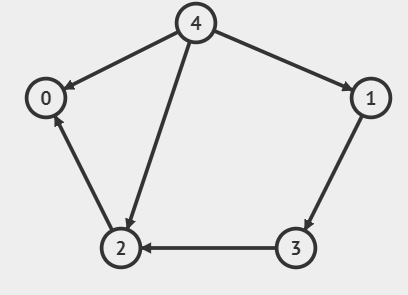
\includegraphics[width=70mm]{example4.png}
\begin{lstlisting}[language=C++]
#include <iostream>
#include "graph.h"

int main()
{
    digraph<int> g;
    g.add_edge(1, 3);
    g.add_edge(2, 0);
    g.add_edge(3, 2);
    g.add_edge(4, 0);
    g.add_edge(4, 1);
    g.add_edge(4, 2);

    
    std::vector<int> V = g.topological_sort();
    std::cout << "The Topological sort is : ";
    for (auto it : V)
    {
        std::cout << it << " ";
    }
    std::cout << std::endl;
    
    return 0;
}

\end{lstlisting}
\\
{\textcolor{black}{\normalsize Output }}
\begin{lstlisting}[language=C++]
The Topological sort is : 4 1 3 2 0 
\end{lstlisting}
\rule{17cm}{0.1mm}
\subsubsection*{\textcolor{blue}{\Large\texttt{digraph::SCCs}}}
Finds all strongly connected components in the given directed graph.



\subsubsection*{\textcolor{blue}{ \large {Syntax}}}
\begin{lstlisting}[language=C++]
std::vector<std::vector<T>> SCCs();

\end{lstlisting}
\subsubsection*{\textcolor{blue}{ \large {Return Value}}}
Returns a list of lists or, more precisely, a vector of vectors containing all SCCs in the given directed graph.
\subsubsection*{\textcolor{blue}{ \large {Algorithm
}}}
It uses Kosaraju's algorithm to find SCCs of the given Directed graph
\begin{enumerate}  
\item Create an empty stack S and do dfs traversal of the graph.
\item  In dfs traversal, after calling the recursive dfs for adjacent vertices of a vertex, push the vertex to the stack. This will store all the vertices in the stack in order of their finishing times.

\item Reverse directions of all edges to obtain the transpose graph.

\item  One by one, pop the top vertex from S while S is not empty. Perform the dfs traversal assuming the popped vertex as source.

\item The dfs starting from the popped vertex will give the strongly connected components of the popped vertex
\end{enumerate}  
\\
\subsubsection*{\textcolor{blue}{ \large {Time Complexity}}}
Since it performs dfs which takes O(V+E) and then reversing the graph also takes O(V+E), so time complexity of this algorithm is O(V+E).

\rule{17cm}{0.1mm}


\subsubsection*{\textcolor{blue}{\Large\texttt{digraph::number\_of\_SCCs}}}
Finds the number of strongly connected components in the given directed graph. It calls digraph::SCCs and returns the size of the vector returned




\subsubsection*{\textcolor{blue}{ \large {Syntax}}}
\begin{lstlisting}[language=C++]
int number_of_SCCs();


\end{lstlisting}
\subsubsection*{\textcolor{blue}{ \large {Return Value}}}
Returns the number of strongly connected components in the given directed graph


\
\\
\rule{17cm}{0.1mm}


\subsection*{\textcolor{blue}{\Large Example }}
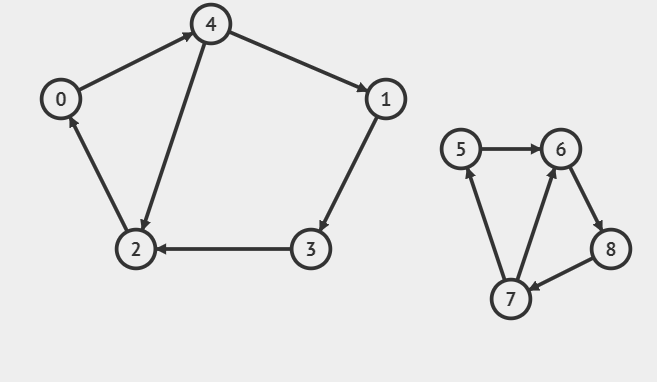
\includegraphics[width=70mm]{example5.png}
\begin{lstlisting}[language=C++]
#include <iostream>
#include "graph.h"

int main()
{
    digraph<int> g;
    g.add_edge(0, 4);
    g.add_edge(1, 3);
    g.add_edge(2, 0);
    g.add_edge(3, 2);
    g.add_edge(4, 1);
    g.add_edge(4, 2);
    g.add_edge(5, 6);
    g.add_edge(6, 8);
    g.add_edge(7, 5); 
    g.add_edge(7, 6); 
    g.add_edge(8, 7); 

    
    std::cout<<"The no. of strongly connected component is "<<g.number_of_SCCs()<<std::endl;
    std::cout<<"The Strongly Connected components are : "<<std::endl;
    std::vector<std::vector<int>> V1 = g.SCCs();
    for (auto i : V1)
    {
        for (auto j : i)
        {
            std::cout<<j<<" ";
        }
        std::cout<<std::endl;
    }

    return 0;
}

\end{lstlisting}
\\
{\textcolor{black}{\normalsize Output }}
\begin{lstlisting}[language=C++]
The no. of strongly connected component is 2
The Strongly Connected components are :
5 7 8 6
0 2 3 1 4
\end{lstlisting}
\rule{17cm}{0.1mm}
\section*{\textcolor{blue}{{\huge \texttt{wgraph} Class}} }
A template container class for weighted undirected graphs. Allows only integer weights to the edges.

\subsection*{\textcolor{blue}{{\LARGE - Members}}}
For number\_of\_nodes, number\_of\_edges, add\_node, remove\_node, remove\_edge, degree, and clear see graph class.


\rule{17cm}{0.1mm}

\subsubsection*{\textcolor{blue}{\Large\texttt{wgraph::adj}}}
Stores the adjacency list of the graph. It is implemented using map data structure in which each node is mapped to a vector of pairs in which the first attribute is the neighbour of that node and the second attribute is the weight of the edge connecting it to that node.






\subsubsection*{\textcolor{blue}{ \large {Syntax}}}
\begin{lstlisting}[language=C++]
std::map<T, std::vector<std::pair<T, int>>> adj;



\end{lstlisting}



\
\\
\rule{17cm}{0.1mm}


\subsubsection*{\textcolor{blue}{\Large\texttt{wgraph::add\_edge}}}
Adds an undirected edge between the two specified nodes with specified weight. Weight must be an integer. If weight is not mentioned, the default weight is used, which is 1.

\subsubsection*{\textcolor{blue}{ \large {Syntax}}}
\begin{lstlisting}[language=C++]
void add_edge(T v, T w, int k);
\end{lstlisting}

\subsubsection*{\textcolor{blue}{ \large {Parameters}}}
u\\
First node
v\\
Second node
k\\
Weight

\subsubsection*{\textcolor{blue}{ \large {Time Complexity}}}
O(log n) where n is the number of nodes



\\
\rule{17cm}{0.1mm}

\subsubsection*{\textcolor{blue}{\Large\texttt{wgraph::bellman\_ford}}}
Finds the shortest distance from every vertex to all other vertices, and also detects negative weight cycle


\subsubsection*{\textcolor{blue}{ \large {Syntax}}}
\begin{lstlisting}[language=C++]
std::vector<std::vector<int> bellman_ford();

\end{lstlisting}

\subsubsection*{\textcolor{blue}{ \large {Return Value}}}
Returns a list of lists or, more precisely, a vector of vectors containing shortest distances from every vertex to every other vertex for the given directed graph.

\subsubsection*{\textcolor{blue}{ \large {Algorithms}}}
Our implementation of bellman ford algorithm is described as follows:
\begin{enumerate}  
\item Perform the following operations for every vertex of the graph taking them as source.

\item Initialise distance from the source to all vertices as infinite and distance to the source itself as zero.


\item Create a map dist which stores all vertices as keys and sets their distances as infinite except dist[src], where src is the source vertex.
\item Do this operation |V| -1 times, it will calculate the the shortest distances.
\item[--] If dist[v] > dist[u] + weight of edge uv, then update dist[v] to dist[v] = dist[u] + weight of edge uv.
\item Again traverse every edge and do following for each u-v 
\item[--]  If dist[v] > dist[u] + weight of edge uv, then graph contains Negative weight cycle


\end{enumerate}  

\\
\rule{17cm}{0.1mm}


\subsubsection*{\textcolor{blue}{\Large\texttt{wgraph::dijkstra}}}
Find the shortest distance between a starting vertex s and all other vertices.


\subsubsection*{\textcolor{blue}{ \large {Syntax}}}
\begin{lstlisting}[language=C++]
std::map<T, int> dijkstra(T s);
\end{lstlisting}

\subsubsection*{\textcolor{blue}{ \large {Parameters}}}
s\\
Starting vertex


\subsubsection*{\textcolor{blue}{ \large {Return Value}}}
Returns a map that maps all vertices to their shortest distance from the starting vertex.
\subsubsection*{\textcolor{blue}{ \large {Remarks}}}
The algorithm will work if and only if the weights of all edges are non-negative.
\subsubsection*{\textcolor{blue}{ \large {Algorithms}}}
Our implementation of dijkstra’s algorithm is described as follows:
\begin{enumerate}  
\item Create a map of predecessors and a map of distances. Initialize the map of distances with infinity (INT\_MAX). Set distance of the starting vertex s from itself as 0.
\item Create a min priority queue q of pairs in which the first attribute is distance from s and the second attribute is a graph node. Initialize it with {0, s}.

\item Extract the v and d\_v (distance of v from s)  from the top of the min priority queue q. If the queue is empty, halt and continue from step 6.
\item If d\_v and d[v] (distance map) are equal, halt and continue from step 3, otherwise continue.
\item For all neighbours e of v, if d[v] + weight of edge {v, e} / (v, e) (for wdigraph) is less than distance of e from s than update the distance of e from s. Push the pair of distance of e from s and e in the priority queue q. Update predecessor of e to v.
\item Finally, return d.

\end{enumerate}  
\subsubsection*{\textcolor{blue}{ \large {Time Complexity}}}
Time complexity depends on finding vertex with smallest distance from s and the time taken for updating distance map. The time complexity is O(E log V).

\\
\rule{17cm}{0.1mm}


\subsubsection*{\textcolor{blue}{\Large\texttt{wgraph::path}}}
Finds the shortest path from a starting node to an ending node



\subsubsection*{\textcolor{blue}{ \large {Syntax}}}
\begin{lstlisting}[language=C++]
std::vector<T> path(T from, T to);

\end{lstlisting}

\subsubsection*{\textcolor{blue}{ \large {Parameters}}}
from\\
Starting node\\
to\\
Ending node\\



\subsubsection*{\textcolor{blue}{ \large {Return Value}}}
Return a vector containing the shortest path from the starting node to the ending node

\subsubsection*{\textcolor{blue}{ \large {Remarks}}}
Its internal implementation uses Dijkstra's algorithm. It calls the function dijksta.

\subsection*{\textcolor{blue}{\Large Example }}
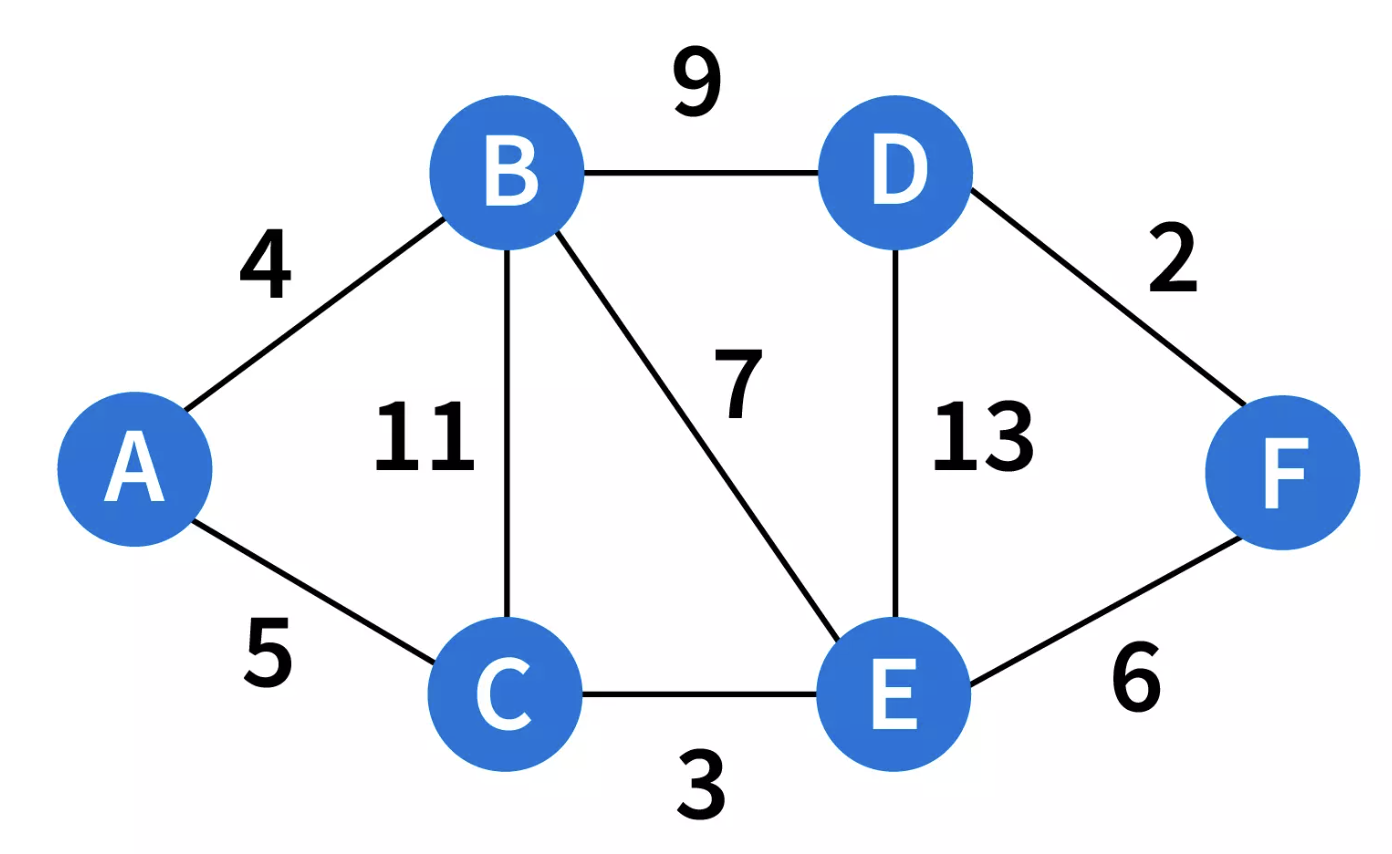
\includegraphics[width=100mm]{example7.png}
\begin{lstlisting}[language=C++]
#include <iostream>
#include "graph.h"

int main()
{
    wgraph<char> g;
    g.add_edge('A', 'B', 4);
    g.add_edge('B', 'D', 9);
    g.add_edge('D', 'F', 2);
    g.add_edge('F', 'E', 6);
    g.add_edge('E', 'C', 3);
    g.add_edge('C', 'A', 5);
    g.add_edge('B', 'C', 11);
    g.add_edge('E', 'D', 13);
    g.add_edge('E', 'B', 7);

    std::cout << "By Dijkshtra's Algorithm.... " << std::endl;
    std::cout << std::endl;

    std::map<char, int> V = g.dijkstra('A');
    std::cout << "Shortest Distance From A to all other nodes : " << std::endl;
    for (auto it : V)
    {
        std::cout << it.first << " : " << it.second << std::endl;
    }
    std::cout<<std::endl;
    std::vector<char> V1 = g.path('A', 'F');
    std::cout << "Shortest Path From A to F is : " ;
    for (auto it : V1)
    {
        std::cout<<it<<" ";
    }
    std::cout<<std::endl;

    return 0;
}

\end{lstlisting}
\\
{\textcolor{black}{\normalsize Output }}
\begin{lstlisting}[language=C++]
By Dijkshtra's Algorithm.... 

Shortest Distance From A to all other nodes :
A : 0
B : 4
C : 5
D : 13
E : 8
F : 14

Shortest Path From A to F is : A C E F
\end{lstlisting}
\rule{17cm}{0.1mm}
\section*{\textcolor{blue}{{\huge \texttt{wdigraph} Class}} }
A template container class for weighted directed graphs. Allows only integer weights to the edges. Allows only integer weights to the edges.

\subsection*{\textcolor{blue}{{\LARGE - Members}}}
For number\_of\_nodes, number\_of\_edges, in\_degree, out\_degree, add\_edge, add\_node, remove\_edge see digraph class.
For bellman\_ford, dijkstra, path see wgraph class.
\\
\rule{17cm}{0.1mm}
\subsubsection*{\textcolor{blue}{\Large\texttt{wdigraph::add\_edge}}}
Adds a directed edge from the first node to the second with a specified weight. Weight must be an integer. If weight is not mentioned, the default weight is used, which is 1.







\subsubsection*{\textcolor{blue}{ \large {Syntax}}}
\begin{lstlisting}[language=C++]
void add_edge(T v, T w, int k);





\end{lstlisting}

\subsubsection*{\textcolor{blue}{ \large {Parameters}}}
u\\
First node\\
v\\
Second node\\
k\\
Weight
\subsubsection*{\textcolor{blue}{ \large {Remarks}}}
Edge is directed from u to v (first node to second). It is assumed that multiple (parallel) edges are not added. The order in which the nodes occur is important.
\subsubsection*{\textcolor{blue}{ \large {Time Complexity}}}
O(log n) where n is the number of nodes

\rule{17cm}{0.1mm}
\subsection*{\textcolor{blue}{\Large Example }}
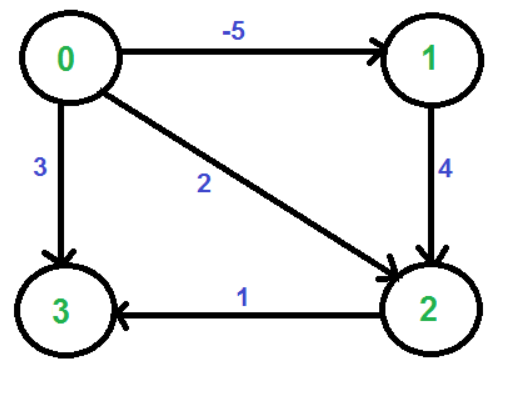
\includegraphics[width=70mm]{example6.png}
\begin{lstlisting}[language=C++]
#include <iostream>
#include "graph.h"

int main()
{
    wdigraph<int> g;
    g.add_edge(0, 1, -5);
    g.add_edge(0, 3, 3);
    g.add_edge(0, 2, 2);
    g.add_edge(2, 3, 1);
    g.add_edge(1, 2, 4);
    
    std::cout<<"By Bellman Ford Algorithm.... "<<std::endl;
    std::cout << std::endl;

    std::vector<std::vector<int>> V = g.bellman_ford();
    std::cout << "Shortest Distance From all nodes to all other nodes : " << std::endl;

    std::cout << std::endl;
    std::cout << "  ";
    for (auto i : g.adj)
    {
        std::cout << i.first << " ";
    }
    std::cout << std::endl;
    auto it = g.adj.begin();
    for (auto i : V)
    {
        std::cout << it->first << " ";
        for (auto j : i)
        {
            if (j == INT_MAX)
            {
                std::cout << "N ";
            }
            else
            {
                std::cout << j << " ";
            }
        }
        std::cout << std::endl;
        it++;
    }
    std::cout << std::endl;

    return 0;
}

\end{lstlisting}
\\
{\textcolor{black}{\normalsize Output }}
\begin{lstlisting}[language=C++]
By Bellman Ford Algorithm.... 

Shortest Distance From all nodes to all other nodes :

  0 1 2 3
0 0 -5 -1 0
1 N 0 4 5
2 N N 0 1
3 N N N 0
\end{lstlisting}
\rule{17cm}{0.1mm}
% \section{Equations}
% \label{sec:eqs}
% This section gives some examples of writing mathematical equations in your thesis.

% Maxwell's equations read:
% \begin{subequations}
%     \label{eq:maxwell}
%     \begin{align}[left=\empheqlbrace]
%     \nabla\cdot \bm{D} & = \rho, \label{eq:maxwell1} \\
%     \nabla \times \bm{E} +  \frac{\partial \bm{B}}{\partial t} & = \bm{0}, \label{eq:maxwell2} \\
%     \nabla\cdot \bm{B} & = 0, \label{eq:maxwell3} \\
%     \nabla \times \bm{H} - \frac{\partial \bm{D}}{\partial t} &= \bm{J}. \label{eq:maxwell4}
%     \end{align}
% \end{subequations}

% Equation~\eqref{eq:maxwell} is automatically labeled by \texttt{cleveref},
% as well as Equation~\eqref{eq:maxwell1} and Equation~\eqref{eq:maxwell3}.
% Thanks to the \verb|cleveref| package, there is no need to use \verb|\eqref|.
% Equations have to be numbered only if they are referenced in the text.

% Equations~\eqref{eq:maxwell_multilabels1}, \eqref{eq:maxwell_multilabels2}, \eqref{eq:maxwell_multilabels3}, and \eqref{eq:maxwell_multilabels4} show again Maxwell's equations without brace:
% \begin{align}
%     \nabla\cdot \bm{D} & = \rho, \label{eq:maxwell_multilabels1} \\
%     \nabla \times \bm{E} +  \frac{\partial \bm{B}}{\partial t} &= \bm{0}, \label{eq:maxwell_multilabels2} \\
%     \nabla\cdot \bm{B} & = 0, \label{eq:maxwell_multilabels3} \\
%     \nabla \times \bm{H} - \frac{\partial \bm{D}}{\partial t} &= \bm{J} \label{eq:maxwell_multilabels4}.
% \end{align}

% Equation~\eqref{eq:maxwell_singlelabel} is the same as before,
% but with just one label:
% \begin{equation}
%     \label{eq:maxwell_singlelabel}
%     \left\{
%     \begin{aligned}
%     \nabla\cdot \bm{D} & = \rho, \\
%     \nabla \times \bm{E} +  \frac{\partial \bm{B}}{\partial t} &= \bm{0},\\
%     \nabla\cdot \bm{B} & = 0, \\
%     \nabla \times \bm{H} - \frac{\partial \bm{D}}{\partial t} &= \bm{J}.
%     \end{aligned}
%     \right.
% \end{equation}

% \section{Figures, Tables and Algorithms}

% Figures, Tables and Algorithms have to contain a Caption that describes their content, and have to be properly referred in the text.

% \subsection{Figures}
% \label{subsec:figures}

% For including pictures in your text you can use \texttt{TikZ} for high-quality hand-made figures \cite{tikz},
% or just include them with the command
% \begin{verbatim}
% \includegraphics[options]{filename.xxx}
% \end{verbatim}
% Here xxx is the correct format, e.g.  \verb|.png|, \verb|.jpg|, \verb|.eps|, \dots.

% \begin{figure}[H]
%     \centering
%     
\includegraphics[width=0.3\textwidth]{Images/IIT_Rpr_logo.jpg}
%     \caption{Caption of the Figure.}
%     \label{fig:quadtree}
% \end{figure}

% Thanks to the \texttt{\textbackslash subfloat} command, a single figure, such as Figure~\ref{fig:quadtree},
% can contain multiple sub-figures with their own caption and label, e.g. Figure~\ref{fig:first_img} and Figure~\ref{fig:second_img}. 

% \begin{figure}[H]
%     \centering
%     \subfloat[One logo.\label{fig:first_img}]{
%         
\includegraphics[width=0.4\textwidth]{Images/IIT_Rpr_logo.jpg}
%     }
%     \quad
%     \subfloat[Another logo.\label{fig:second_img}]{
%         
\includegraphics[width=0.4\textwidth]{Images/IIT_Rpr_logo.jpg}
%     }
%     \caption[]{Caption of the Figure.}
%     \label{fig:quadtree2}
% \end{figure}

% \subsection{Tables}
% \label{subsec:tables}

% Within the environments \texttt{table} and  \texttt{tabular} you can create very fancy tables as the one shown in Table~\ref{table:example}.

% \begin{table}[H]
%     \caption*{\textbf{Example of Table (optional)}}
%     \centering 
%     \begin{tabular}{|p{3em} c c c |}
%     \hline
%     \rowcolor{newblue!40}
%      & \textbf{column1} & \textbf{column2} & \textbf{column3} \T\B \\
%     \hline \hline
%     \textbf{row1} & 1 & 2 & 3 \T\B \\
%     \textbf{row2} & $\alpha$ & $\beta$ & $\gamma$ \T\B\\
%     \textbf{row3} & alpha & beta & gamma \B\\
%     \hline
%     \end{tabular}
%     \\[10pt]
%     \caption{Caption of the Table.}
%     \label{table:example}
% \end{table}

% You can also consider to highlight selected columns or rows in order to make tables more readable.

% \subsection{Algorithms}
% \label{subsec:algorithms}

% Pseudo-algorithms can be written in \LaTeX{} with the \texttt{algorithm} and \texttt{algorithmic} packages.
% An example is shown in Algorithm~\ref{alg:var}.
% \begin{algorithm}[H]
% \label{alg:example}
% \caption{Name of the Algorithm}
% \label{alg:var}
% \label{protocol1}
% \begin{algorithmic}[1]
% \STATE Initial instructions
% \FOR{$for-condition$}
% \STATE{Some instructions}
% \IF{$if-condition$}
% \STATE{Some other instructions}
% \ENDIF
% \ENDFOR
% \WHILE{$while-condition$}
% \STATE{Some further instructions}
% \ENDWHILE
% \STATE Final instructions
% \end{algorithmic}
% \end{algorithm} 


\section*{\textcolor{red}{Applications} }
\begin{enumerate}
    \item  Used for solving flow problems, which encompass real life scenarios like the scheduling of airlines.\\
    \item Directions in a google map works on the concept of finding shortest path using Dijkstra's algorithm\\
    \item Graph Coloring concept can be used to solve the most popular puzzle game, Sudoku and many other board games by converting the board/puzzle into a graph.\\
    \item Search engines such as Google let us navigate through the World Wide Web without any problem using graph theory by first creating a web graph
    \\
\end{enumerate}
\section*{\textcolor{red}{Conclusions}}
\color{black}
In this project, we have created a library which provides data structures for graphs, digraphs, weighted graphs and related algorithms. It will be very useful for studying and analyzing sparse graphs. It can be used to simulate  graphs problems such as Sudoku, Snakes \& Ladders and many other real life problems.

\section*{\textcolor{red}{Bibliography and citations}}
\section*{\textcolor{blue}{Acknowledgements}}
We wish to thank our instructor, Dr Anil Shukla and our Teaching Assistant Sravanthi Chede for their guidance and valuable inputs provided during the project.

\nocite{DiGraphs}
\nocite{wiki}
\nocite{algorithms}
\nocite{graphs}
\nocite{software}

\bibliography{bibliography.bib}

\end{document}